\documentclass{article}
\usepackage{aaai}
\usepackage{fixbib}
\usepackage{amsmath}
\usepackage{graphicx}
\usepackage{times}
\usepackage{helvet}
\usepackage{courier}
\usepackage{graphicx}
\usepackage{multirow}
\usepackage{verbatim}
\usepackage{url}
\usepackage[utf8]{inputenc}
\DeclareUnicodeCharacter{FB01}{fi}
\graphicspath{ {images/} }
\frenchspacing
\setlength{\pdfpagewidth}{8.5in}
\setlength{\pdfpageheight}{11in}


\title{
	CS4246 AI Planning and Decision Making - Project 2 \\
	Planning and Decision Making Automation on Depression
}
\author{
	{\bf Team 01} \\
	Antoine Charles Vincent Garcia - A0159072A\\
	Chan Jun Wei - A0112084U\\
	Chen Tze Cheng - A0112092W\\
	Eric Ewe Yow Choong - A0112204E\\
	Han Liang Wee, Eric - A0065517A\\
	Ho Wei Li - A0094679H\\
}

\begin{document}
 	\maketitle

	\begin{abstract}
	\begin{quote}
	Depression is a debiliatating mental illness that has good prognosis given early detection and treatment. 
	However, detection is difficult with the various factors that raise the entry barriers and decrease the accuracy of a diagnostic test. Research have shown that accurate predictions of emotions can be made with Gaussian Process models. 
	This study explores the novel use Gaussian Process in predicting depression severity using acoustic measures of voice.
	Our work has succesfully shown that Gaussian Process Dot Product trained using MFCC feature set is a good model for depression prediction and can predict PHQ-8 better than other state-of-the-art models at RMSE of 6.34.\\
	\end{quote}
	\end{abstract}
	
	\section{Introduction}
	Depression has a severe, and at times long-term, negative impact on an individual's quality of life. 
	Major depression is 3rd leading cause of disability worldwide with 65 million life years spent living with the disability or lost due to early death \cite{who2004}.
	Depression's annual toll on U.S businesses amounts to about \$80 billion in medical expenditures, lost productivity and suicide. 
	Among the costs, close to \$10 billion accrued in lost workdays each year and more than \$33 billion in other costs accrue from decreased productivity due to symptoms that sap energy, affect work habits, cause problems with concentration, memory, and decision-making \cite{tjcp2015}. \\

	Left unchecked, depression increases risk for morbidity, suicide, decreased cognitive and social functioning, self-neglect, and early death \cite{arcp2009}. 
	Death from suicide is one of the top 10 causes of death, above the death rate for chronic liver disease, Alzheimer's, homicide, arteriosclerosis or hypertension \cite{nvsr2016}. \\

	Despite the severe consequences, depression is one of the most treatable mental illnesses but it is also one of the most under-diagnosed globally. 
	In general health-care, 48.4\% of patients suffering from depression go unrecognized \cite{jama2003}.

	\subsection{Motivation and Objective}
	The Personal Health Questionaire depression scale (PHQ-8) is a self-administered, 8-question diagnostic test for depressive disorders that has proven to be an effective severity measure for depression in large clinical studies \cite{jad2008}. 
	Nevertheless, one of the biggest obstacles to successful diagnosis of depression is the unwillingness of patients to admit their predisposition to depression by seeking help.\\

	People often subscribe to the social stigma that being depressed reflects a weakness in their character, a permanent defect in their personality. 
	This stigma manifests itself particularly in a phenomenon known as social distancing whereby people with mental issues are more isolated from others \cite{tpcrp2011}.  
	People suffering from depression hence tend to be ashamed of their condition and are generally convinced that denying and hiding it from others gives them a better shot at integrating with society and living a normal life \cite{bmb2001}.
	Even if they do seek help, the accuracy of the PHQ-8 or just questionaires and surveys in general are often adversely affected by the Hawthorne Effect, 
	a type of reactivity in which individuals modify or improve an aspect of their behavior in response to their awareness of being observed. \cite{jce2014}.\\

	In the past decade, there have been research successfully correlating emotion with voice production and speech acoustics \cite{uwa2001}. 
	Corollary to that, active research of late into the use of voice acoustics as predictors of clinical depression scores has seen success, proving that it is an effective indicator of depression severity \cite{jov2016}.\\

	In this paper, we investigate the applicability and feasibility of Gaussian Process (GP) models in predicting clinical ratings of depression severity on the PHQ-8 scale with acoustic measures of voice from a sample of patients and compare their performance with current state-of-the-art machine learning models. 
	Some of our preliminary studies have shown that despite consensus among the scientific community that Support Vector Machine (SVM) models have a 
	very high predictive accuracy specifically in speech emotion recognition \cite{Chavhan2010}, GP models have been proven to consistently outperform SVM models on the task of music emotion recognition \cite{MARKOV2013}. 
	Nevertheless, there are no studies on the use of GP in predicting depression severity. 
	The findings of this paper will hopefully open up new frontiers and fuel further research interest on this topic.
	
	\subsection{Important Requirements}
	...
	
	\section{Modelling and Approach}
	As  stated in the Future Applications subsection of Project 1, we replicate a similar application which not only offers higher accessibility, more user-friendly approach and reduced social stigma, but in addition, to give a reasonable and acceptable prediction of users' depression levels. \\	
	
	The following premises have to hold true so that the GP model planning and decision making is suitable for depression prediction:
	\begin{enumerate}
		\item Depression prediction is an event-based recognition which provides a single depression estimate over a certain amount of time. \cite{Valstar2016}
		\item The speech signals extracted from different people suffering from depression should share some similarities and thus admissible for prediction with the Gaussian Process models. 
		For example, diminished, prosodic and monotonous speech is often strongly correlated with depression \cite{Cummins2015}.
	\end{enumerate}

	\subsection{Qualitative Advantages}
	As seen in our Motivation and Objective section of Project 1, good prognosis comes with early detection of depression. 
	Although it is known that depression or rather emotions is general, are subjective and is difficult to predict, the capability of GP in retrieving the confidence intervals of the prediction and a continuous measurement over time may offset the uncertainty.
	Accurate prediction is essential to not only licensed authorities but will also help more users to harbour acceptance towards their affliction to seek medical attention.
	In addition, planning and decision making is also inline with our Future Applications subsection in Project 1 and thus, extending from there allows us to demonstrate the high feasibilty of our experiment.
	
	\subsection{Planning and Decision Making} \label{pdm}
	In our previous report, we have demonstrated that we are able to predict depression with GP. 
	With the data obtained, we will extend our experiment to demonstrate how our model can plan and make decisions accordingly. \\
	
	\subsection{Reinforcement Learning (RL)}
	...

	\subsection{Modifications and Additional Insights}
	...

	\section{Evaluation}
	In order to test our proposed GP models, we conducted tests on data obtained from Audio/Visual Emotion Challenge and Workshop (AVEC 2016) \cite{avec2016}. 
	The goal of AVEC is to weigh-in on the various approaches used to recognize emotions under unambiguous conditions. 
	AVEC 2016 provided 2 pieces of data as input: visual and auditory data from each of the participants. 
	However, we would be reducing the scope of the experiment, limiting the experiment to only the auditory data. 
	Two Sub-Challenges were lised in AVEC 2016. 
	We are only interested in the Depression Classification Sub-Challenge, which requires participants to classify inputs by the PHQ-8 score. 
	In this experiment, we would be using the audio data along with their corresponding PHQ-8 scores to test our assumptions and confirm our hypothesis.

	\subsection{Data}
	\begin{figure}[h]
	\center
 	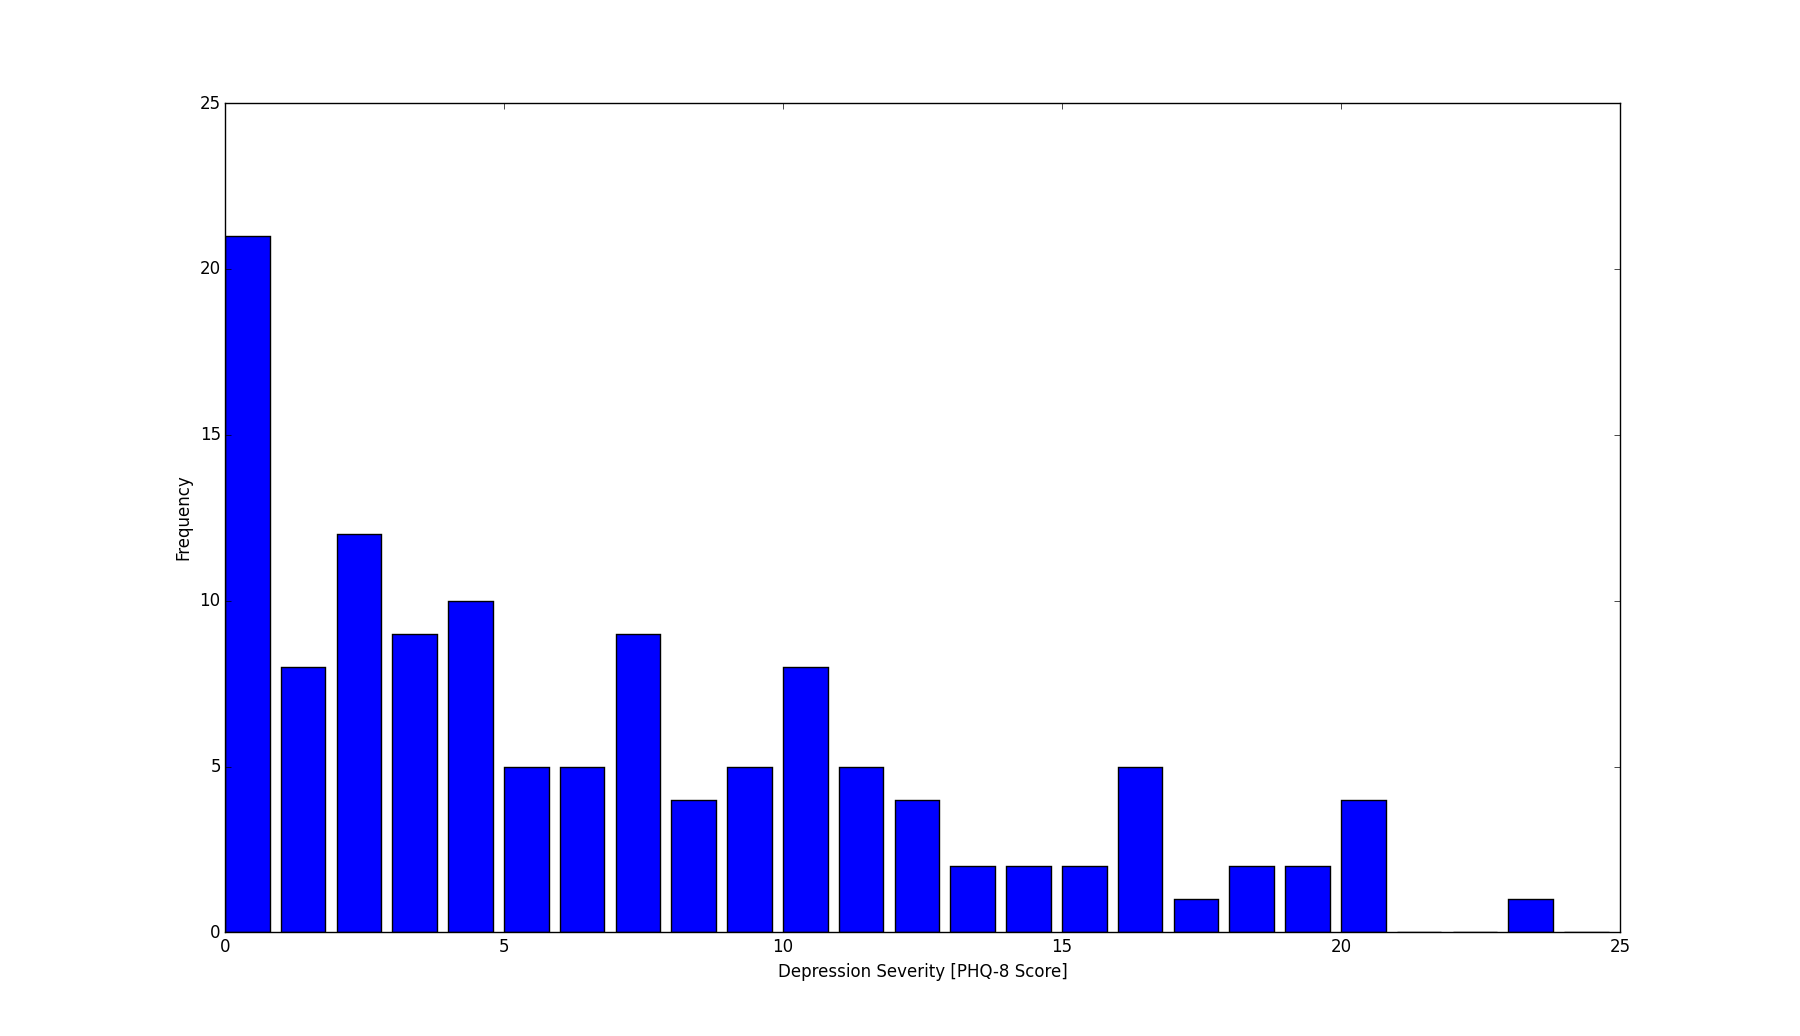
\includegraphics[width=0.5\textwidth]{histogram_phq8}
	\caption{Histogram of the PHQ-8 scores}
	\label{histogram_phq8}
	\end{figure}
	
	The depression data used in AVEC 2016 was obtained from the benchmarking database, Distress Analysis Interview Corpus - Wizard of Oz (DAIC-WOZ). 
	Data collected from DAIC-WOZ include raw audio and video recordings and the corresponsing PHQ-8 score (from 0 to 24) \cite{jad2008}. Hence, we would 
	need to pre-process the auditory data before we use it in our experiment. The pre-processing is briefly discussed in the section below.
	The distribution of the depression severity scores in the dataset is given in Figure \ref{histogram_phq8}. 
	The data provided are split into 2 sets: training and development.
	An overview of the data is given in Table \ref{summary_table}.

 	\begin{table}[h]
 		\begin{center}
  			\begin{tabular}{ | r | c | c | c | }
    			\hline
			 		& \bfseries Training	& \bfseries Development 	& \bfseries All \\ \hline
			 $n$		& 95 			& 31 				& 126 \\ \hline
			 $\mu$	& 6.326 		& 7.548			& 6.626 \\ \hline
			 $\sigma$	& 5.597 		& 6.690 			& 5.909 \\ \hline
			 \end{tabular}
		\end{center}
 	\caption{Summary of Datasets provided}
 	\label{summary_table}
 	\end{table}

	\subsection{Pre-processed data}
	Since the focus of this paper is the prediction of the PHQ-8 score, we will not describe the pre-processing step in detail.
	We used standard signal processing techniques to extract the 4 audio feature sets (Energy, MFCC, Magnitude Spectrum, Zero-crossing) as presented in the Modelling 
	and Approach section.
	Each audio feature set comprises of several individual features and the breakdown of the actual number of feature columns is summarized in Table \ref{no_features}.

 	\begin{table}[h]
 		\begin{center}
  			\begin{tabular}{ | r | c | }
    			\hline
			 \bfseries Audio Feature Sets 	& \bfseries Number of features \\ \hline
			 Magnitude Spectrum		& 512 \\ \hline
			 MFCC 				& 12 \\ \hline
			 Energy 				& 1 \\ \hline
			 Zero-Crossing Rate 		& 1 \\ \hline
			 \bfseries Total			& \bfseries 526 \\ \hline
			 \end{tabular}
		\end{center}
 	\caption{Number of features extracted}
 	\label{no_features}
 	\end{table}

 	\subsection{Measure of Accuracy}
	AVEC 2016 provided a baseline classifier that consistently predicts the PHQ-8 score with $\text{RMSE}=6.7418$ \cite{avec2016}. 
	In order to provide a meaningful and consistent comparison to the baseline provided, we used the same Root Mean Square Deviation Error (RMSE) to measure the 
	error rate on both Training and Development datasets. 
	RMSE (Equation \ref{eq:rmse}) is a commonly used in the machine learning community to measure the differences between the values predicted by a model 
	and the ground truth \cite{Dhanani:EECS-2014-131}. 
	\begin{equation}\label{eq:rmse}
  	\text{RMSE} = \sqrt{\frac{\sum_{t=1}^n (\hat y_t - y_t)^2}{n}}
 	\end{equation} 

	\subsection{Feature Selection}
	Feature selection is the process of selecting a subset of relevant features including variables or predictors to be used in a model for machine learning. 
	The purpose of feature selection is to reduce the complexity of a model to more easily be interpreted. 
	The benefit is three-fold: improving the prediction performance of the predictors, providing faster and most cost-effective predictors, 
	and providing a better understanding of the underlying process that generated the data \cite{Guyon2003}.\\
	
	Since we have more features than data points, it tends to lead to overfitting \cite{Smith2011}. 
	Therefore feature selection is first performed on the data before applying machine learning. 
	The feature selection algorithms used are popular and are taken from scikit-feature, a feature selection library \cite{li2016feature}: CIFE \cite{Lin2006}, Relief 	
	\cite{Rob2003}, CFS \cite{HALLHALL}. 
	We will not go into detail as feature selection is not the main focus of the report.
	
	\subsection{Experimental Setup}
	We compared the proposed GP models against state-of-the-art machine learning models as mentioned in the previous section. 
	For the ease of testing, all implementations of the algorithms except for GP ARD come from the popular machine learning library, Scikit Learn \cite{scikit-learn}. 
	We used the implementation of GP ARD from GPy, a Gaussian Processes framework in Python \cite{gpy2014}.
	The hyper-parameters are either determined by the defaults used in either libraries or some reasonable defaults were used.
	Each machine learning model is trained against the training set and thereafter tested against the development set using RMSE as the error metric. 
	The entire experimental process is shown in Figure \ref{process}. \\
 
 	\begin{comment}
	\begin{table}[h]
  		\begin{center}
   			\begin{tabular}{ | r | c |}
	    		\hline
			Algorithm & Hyper-parameters \\ \hline\hline
			K-Nearest Neighbors        & x \\ \hline
			SVM - Linear               & x \\ \hline
			SVM - RBF                  & x \\ \hline
			Decision Tree              & x \\ \hline
			Random Forest              & x \\ \hline
			AdaBoost                   & x \\ \hline
			Naive Bayes                & x \\ \hline
			GP ARD  	           & x \\ \hline
			GP Isotropic Matern        & x \\ \hline
			GP Dot Product 	           & x \\ \hline
			\end{tabular}
		\end{center}
		\caption{List of Machine Learning Algorithms with their corresponding hyper-parameters}
		\label{list_mls}
	\end{table}
 	\end{comment}
 	
	\begin{figure}[h]
 		\begin{center}
		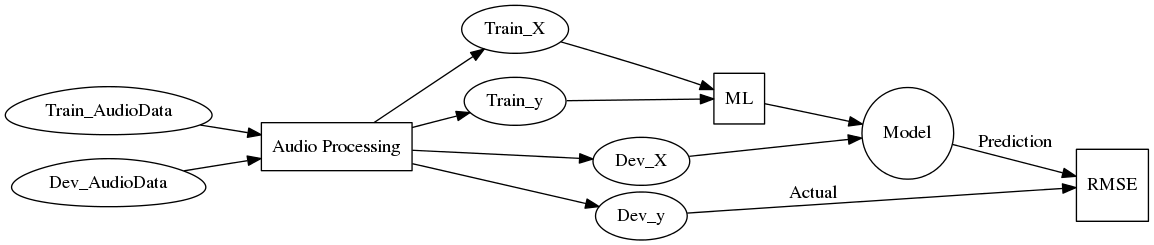
\includegraphics[width=0.48\textwidth]{process} 
  		\end{center}
  		\caption{Experimental process}
  		\label{process} 
 	\end{figure}
 	\begin{comment}
	@startuml
	digraph g {
		graph [rankdir=LR];
	 	ML,RMSE[shape=square];
		Model[shape=circle];
		ap[shape=rect label="Audio Processing"];
		Train_AudioData,Dev_AudioData[shape=egg];
		Train_AudioData -> ap;
		ap -> Train_X;
		ap -> Train_y;
		ap -> Dev_X;
		Dev_AudioData -> ap;
		ap -> Dev_y;
		Train_X -> ML;
		Train_y -> ML;
		ML -> Model
		Dev_X -> Model
		Model -> RMSE[label=Prediction]
		Dev_y -> RMSE[label=Actual]
	}
	@enduml
 	\end{comment}

	\subsection{Results}
	We first ran the experiment across the dataset using all 526 features, without feature selection. 
	As we would expect \cite{Cawley2014}, the results are unacceptable as the ratio of the number of features to the number of data points is too high,
	resulting in possible overfitting. 
	The results of the initial experiment is illustrated in Figure \ref{results_all}. 
	We would expect the GP ARD would be able to theoritcally extract relevant features and improve prediction.
	However, we have observed experimentally that GP ARD performs poorly, along with other GPs. \\

	\begin{figure}[h]
 		\begin{center}
		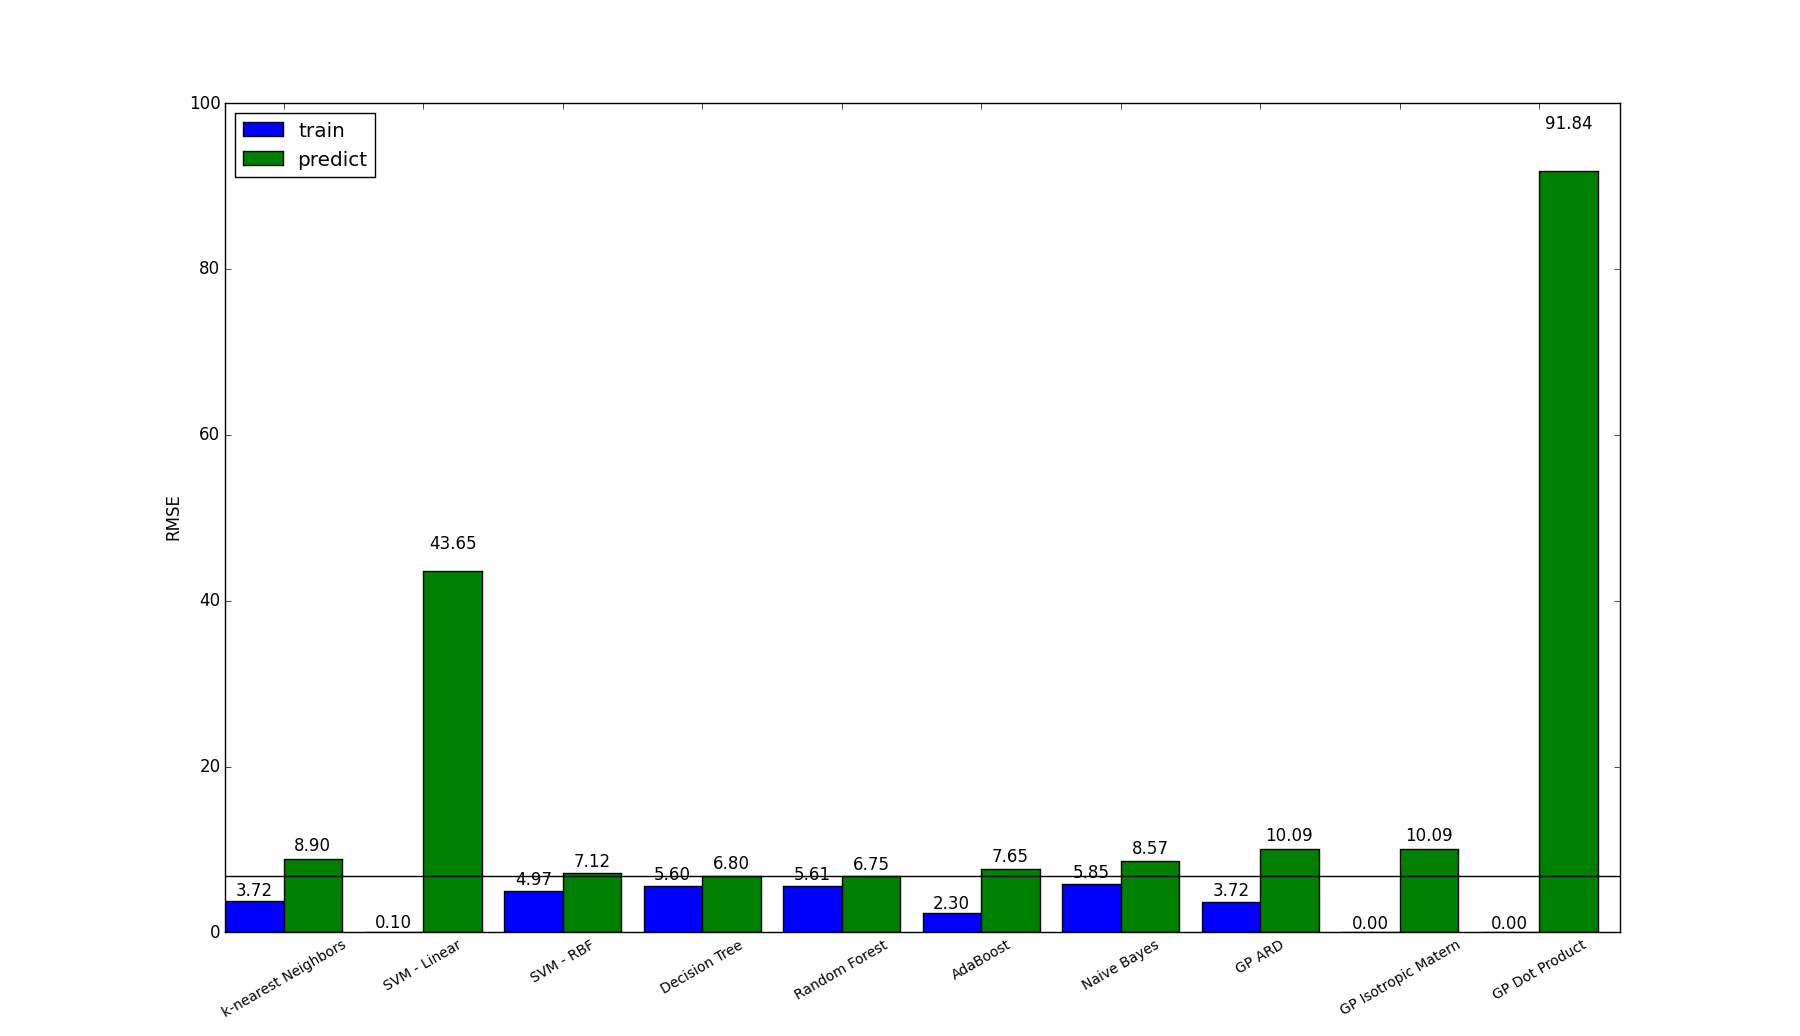
\includegraphics[width=0.5\textwidth]{results_all} 
  		\end{center}
  		\caption{Results across all features}
  		\label{results_all}
 	\end{figure}
	
	We repeated the experiment with feature selection and ran each of the feature subset gathered from the feature selection algorithms against each of the machine 
	learning algorithms. 
	We observed that Relief, CIFE and CFS selected a large number of MFCC features. 
	The number of features in each feature subset is shown in Table \ref{feat_subset}. 
	This confirms our assumption that MFCC gives the best predictive power in PHQ-8 depression severity prediction. 
	Hence, we also ran the experiment using only MFCC features. 
	The best results across all feature subsets are shown in Figure \ref{results_best} and in Table \ref{rmse_results}. The line shown across the 
	bar chart represents the baseline RMSE provided. \\

 	\begin{table}[h]
 		\begin{center}
  			\begin{tabular}{ | r | c | }
    			\hline
			 \bfseries Feature Selection 	&\bfseries Number of features \\ \hline
			 MFCC           			& 12 \\ \hline
			 CIFE        				& 3 \\ \hline
			 Relief 				& 23 \\ \hline
			 CFS 					& 6 \\ \hline
			 All 					& 526 \\ \hline
			 \end{tabular}
		\end{center}
 	\caption{Feature subsets}
 	\label{feat_subset}
 	\end{table}

	\begin{figure}[h]
 		\begin{center}
		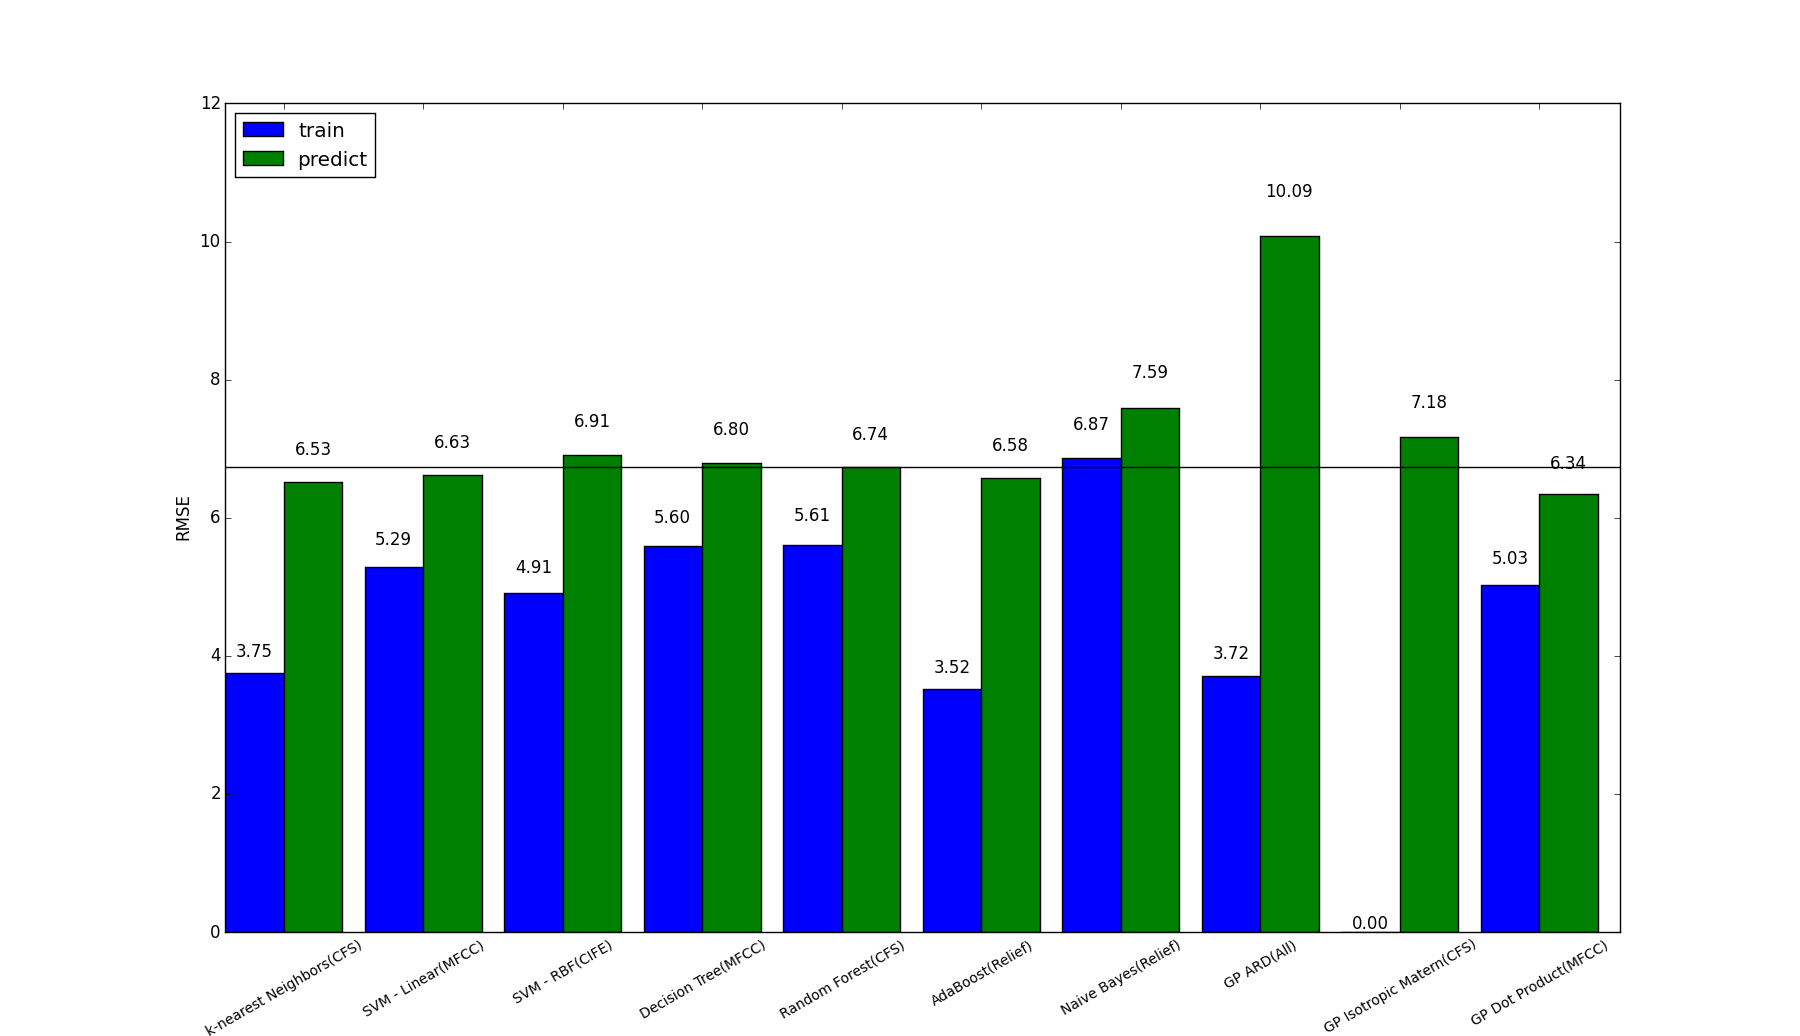
\includegraphics[width=0.5\textwidth]{results_best} 
  		\end{center}
  		\caption{Best Results across all feature subsets}
  		\label{results_best}
 	\end{figure}

	\begin{table}[h!]
		\begin{center}
			\begin{tabular}{ | r | c | c | c | }
			\hline
			\multirow{2}{*}{\bfseries Algorithm}	& \multirow{2}{*}{\bfseries Subset}	& \multicolumn{2}{c|}{\bfseries RMSE} \\\cline{3-4}
									&						& \bfseries Train 	& \bfseries Dev \\ \hline
			\bfseries GP Dot Product  	& \bfseries MFCC  & \bfseries 5.03 & \bfseries 6.34 \\ \hline
			AdaBoost              				& Relief					& 3.55 		& 6.52 \\ \hline
			K-Nearest Neighbors   			& CFS 					& 3.75 		& 6.53 \\ \hline
			SVM - Linear          				& MFCC  					& 5.29 		& 6.63 \\ \hline
			Random Forest         			& CFS   					& 5.61 		& 6.75 \\ \hline
			Decision Tree         				& MFCC  					& 5.60 		& 6.80 \\ \hline
			SVM - RBF             				& CIFE  					& 4.91 		& 6.91 \\ \hline
			GP Isotropic Matern   			& CFS   					& 0.00 		& 7.18 \\ \hline 
			Naive Bayes           				& Relief					& 6.87 		& 7.59 \\ \hline
			GP ARD                				& All   						& 3.72 		& 10.09 \\ \hline

			\end{tabular}
		\end{center}
		\caption{RMSE Results}
		\label{rmse_results}
	\end{table}
	
	As expected, the models perform better with the MFCC feature set. 
	Unexpectedly, the simple GP dot product model, trained with 12 features and 95 data points, outperforms all other machine learning models in our tests. 
	Our results also confirms the initial assumption that MFCC is an appropriate feature set to be used in emotion and therefore depression prediction and that GP is 
	applicable and feasible in predicting PHQ-8 scores.

	Here are the 95\% confidence interval for the predicted PHQ8 score for each subject of the test set.

	\begin{figure}[h]
 		\begin{center}
		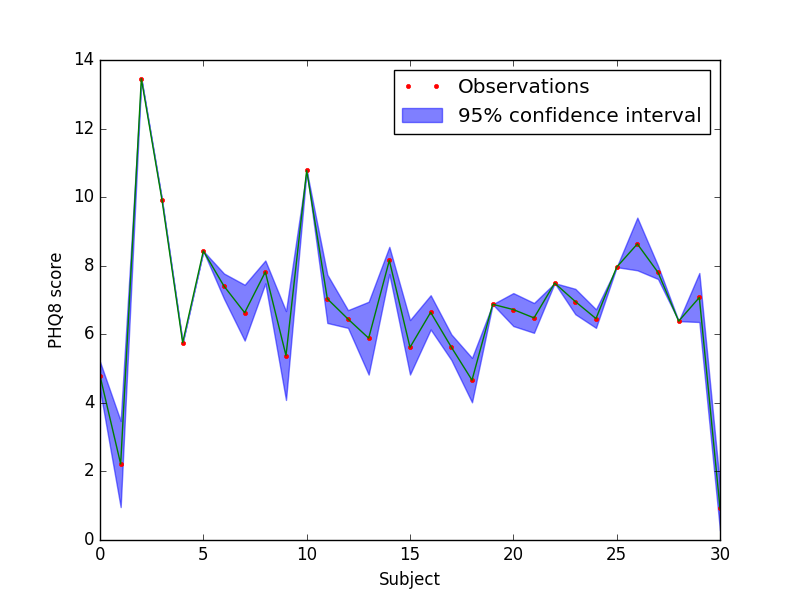
\includegraphics[width=0.5\textwidth]{Confidence}
  		\end{center}
  		\caption{Confidence interval for each subject of the test set}
  		\label{Confidence}
 	\end{figure}

	\section{Conclusion}	
	Our work has succesfully shown that GP is a good model for this problem and can predict PHQ-8 better than state-of-the-art machine learning models. 
	In addition to being on par or better at prediction, GP can inherently provide an estimate of prediction uncertainty. 
	This allows the user to gauge the model's confidence of the prediction, and to make more informed decisions based on both the prediction and its uncertainty. 
	We can also intelligently supplement more data to our training set based on the prediction uncertaintly. 
	Therefore, after considering both results and GP's advantages, we conclude the GP Dot Product trained using MFCC feature set is a good model for 
	depression prediction.
	
	\section{Further Work}
	For this experiment, we only used machine learning algorithms with their default parameters. 
	An aspect that deserves further exploration is to perform automatic hyper-parameter optimization
	across all the machine learning algorithms to fine-tune each model's performance. 
	In particular, we can try Hyperopt-sklearn \cite{Komer2014HyperoptsklearnAH} or GP based hyper-parameter tuner. 
	We opine that with hyper-parameter tuning, we can predict PHQ-8 scores better and can have a more objective comparison of the different learning algorithms.
	
	\section{Contributions}
	\begin{itemize}
		\item \textbf{Antoine Charles Vincent Garcia}: 
		Scripting the program, setting up machine learning libraries, running tests and generation of the utility function.
		\item \textbf{Chan Jun Wei}: 
		Scripting the program, setting up machine learning libraries, running tests and generation of the utility function.
		\item \textbf{Chen Tze Cheng}: 
		Scripting the program, setting up machine learning libraries, running tests and generation of the utility function.
		\item \textbf{Eric Ewe Yow Choong}: 
		Formatting the report as well as research and writing up of the technical approach section.
		\item \textbf{Han Liang Wee, Eric}: 
		Retrieving data, testing as well as research and writing up of the technical approach section.
		\item \textbf{Ho Wei Li}: 
		Research, vetting of the report and writing up of the motivation and introduction of the experiment. \\
	\end{itemize}
	
	\bibliographystyle{aaai}
	{\scriptsize \bibliography{references}}

\end{document}
